\documentclass[11pt]{article}
\usepackage[preprint]{acl}
\hypersetup{pdftitle={Tokenizer Tax and Downstream Performance in Twelve African Languages},
  pdfauthor={Christophe Mumaragishyika},
  pdfkeywords={tokenization, African languages, sentiment analysis, AfriSenti, Kinyarwanda, Swahili}}
\usepackage{times}
\usepackage{latexsym}
\usepackage[T1]{fontenc}
\usepackage[utf8]{inputenc}
\usepackage{microtype}
\usepackage{amsmath,amssymb}
\usepackage{graphicx}
\usepackage{booktabs}
\usepackage{textcomp}

\begin{document}

\title{Tokenizer Tax and Downstream Performance in Twelve African Languages}

\author{Christophe Mumaragishyika \\
  Data Science and Analytics \\
  University of Missouri, Columbia, MO, USA \\
  \texttt{cmmnh@missouri.edu}}

\maketitle

\begin{abstract}
Subword tokenizers built on English-centered data split words of African languages into many pieces, a cost called the token tax. I ask whether this tax predicts the benefit of pretrained models over a bag-of-words baseline in sentiment classification. TF-IDF with logistic regression, frozen LaBSE embeddings with the same classifier and fine-tuned AfroXLMR-base ran with identical settings on the twelve AfriSenti languages with training splits. Fine-tuning beats TF-IDF in four languages, loses in five and ties in three. The test fixed before the runs, Spearman's $\rho$ between subword tokens per word and the fine-tuning gain, is 0.00 (95 percent interval $-0.72$ to $0.69$), and stays near zero under four word definitions and with training size fixed. Pretraining coverage and training size separate the languages better: the two languages absent from every pretraining list lose the most. An audit of the released splits finds artifacts the models can see, among them lower-cased Nigerian test sets and placeholders present in one split only; a placeholder added to the Swahili test set costs both encoders 8.4 and 8.6 macro F1 points. On a 66-item adversarial suite, no pipeline reads a polite formal complaint as negative, and in Kinyarwanda only the encoders read negation.
\end{abstract}

\section{Introduction}
A subword tokenizer trained mostly on English and a few large languages breaks a Kinyarwanda word into about three pieces, roughly double what it does to an English word, as I found in a preliminary measurement and as several studies have reported for other languages \citep{rust2021tokenizer,petrov2023unfairness,ahia2023cost}. The cost has a name, the token tax \citep{lundin2026tokentax}: more pieces per word mean longer inputs, higher API prices, and, in the study that coined the name, lower accuracy of large language models on a multiple-choice benchmark in sixteen African languages.

The question of this paper is narrower and comes from a result of my own. In a preliminary single-language study I compared three sentiment pipelines on the Kinyarwanda part of AfriSenti \citep{muhammad2023afrisenti}: TF-IDF with logistic regression, frozen LaBSE sentence embeddings \citep{feng2022labse} with the same classifier, and AfroXLMR-base \citep{alabi2022adapting} fine-tuned on the training tweets. The fine-tuned model beat TF-IDF by six macro F1 points. That is one language, one dataset, and one vocabulary. If the token tax is what limits pretrained models on African languages, the gain over a lexical baseline should shrink as the vocabulary fragments the language more. If something else limits them, the gain should follow that something else.

I therefore ran the same three pipelines, with identical settings and seeds, on the twelve AfriSenti languages that have training splits, measured for each language how many subword tokens its words take under the two pretrained vocabularies, and tested, with a test fixed before the runs, whether that fertility predicts the gain of fine-tuning over TF-IDF. On the way the data itself asked for attention. The released splits of several languages differ from each other in ways that have nothing to do with sentiment, so I audited them and measured what the differences cost. The contributions are:
\begin{enumerate}
\item Test macro F1 of the three pipelines on twelve languages, with three seeds for the fine-tune and paired bootstrap intervals on every pairwise difference (Section~\ref{sec:results}).
\item The pre-specified test of fertility against the fine-tuning gain, with a permutation $p$-value, a bootstrap interval over languages, a partial version given training size, and a sensitivity check over four word definitions; the answer is no detectable effect.
\item An audit of the AfriSenti release: near-copies between training and test, letter case, script mix and anonymization placeholders per split, with the effect of the mismatches measured on the kept models.
\item Two robustness tests with native-speaker judgment: a Kinyarwanda test set retyped with texting rules, and a 66-item adversarial suite in Kinyarwanda and Swahili whose items and labels were committed before any model scored them.
\item Training time, memory and latency for the three pipelines, as deployment guidance by pretraining coverage.
\end{enumerate}

\section{Related Work}
\citet{rust2021tokenizer} tied the fertility of a multilingual tokenizer, its subword tokens per word, to the monolingual performance of multilingual models on nine languages and showed that a dedicated tokenizer recovers part of the gap. \citet{petrov2023unfairness} showed that the same text costs far more tokens in some languages than in others under the tokenizers of current language models, and \citet{ahia2023cost} turned that into a cost of use for commercial models. \citet{lundin2026tokentax} measured fertility and accuracy for ten large language models on AfriMMLU in sixteen African languages, Swahili among them and Kinyarwanda not, and report that each additional token per word reduces accuracy by 8 to 18 percentage points on average, while noting that fertility is confounded with the availability of training data. Those studies measure either the pretraining of a model or the accuracy of a frozen large model. This paper measures a different quantity: the benefit of a pretrained encoder over a lexical baseline when both are trained on the same labeled tweets. Fertility could act on that quantity through the vocabulary, or not at all.

AfriSenti \citep{muhammad2023afrisenti} is a Twitter sentiment benchmark for fourteen African languages, annotated by three native speakers per tweet with the majority label kept, and released with its per-language agreement. Its four Nigerian-language sets come from NaijaSenti \citep{muhammad2022naijasenti}, which describes how those tweets were collected: queries built from stopwords, emoji and sentiment lexicons, a lexicon filter, retweets and duplicates removed, and lower-casing. Those two descriptions matter for the audit in Section~\ref{sec:audit}. AfroXLMR \citep{alabi2022adapting} adapts XLM-R \citep{conneau2020xlmr} to seventeen African languages by continued pretraining; LaBSE \citep{feng2022labse} is a sentence encoder trained on 109 languages. The lists of languages in those three papers define the coverage classes of Section~\ref{sec:data}.

\section{Data}
\label{sec:data}
\subsection{AfriSenti}
AfriSenti has training splits for twelve of its fourteen languages; Oromo and Tigrinya are test-only and are left out. I loaded the twelve from the parquet conversion of the dataset on the Hugging Face Hub on 26 September 2026 (datasets 5.0.0, with the commit pinned): 106,828 tweets, 63,685 in training, 12,932 in validation and 30,211 in test. The parquet copy has the same number of rows as the released files in all 36 splits; the dataset card, which counts header lines, lists 1,216 Moroccan Arabic validation tweets where the release has 494. Each tweet carries one of three labels, positive, neutral or negative, and the label order of the class feature was checked in every language. The annotation agreement reported by the AfriSenti paper (its Table 5) ranges from 0.41 for Algerian Arabic to 0.66 for Hausa, with 0.43 for Kinyarwanda and no value for Swahili.

\subsection{Normalization and splits}
The normalization is the one of the preliminary study, applied to every language: runs of repeated \texttt{@user} mentions collapsed to one, links replaced by the token \texttt{http}, whitespace collapsed, and one rule added here, a pair of straight quotes wrapping a whole tweet removed, which touched all 1,999 Amharic test tweets and nothing else (a file artifact, not language). Emoji, hashtags, apostrophes and hyphens are kept; an ablation in that study found no measurable effect of the two marks ($-0.3$ macro F1 points, 95 percent paired bootstrap interval $-1.4$ to $+1.0$). Training rows whose normalized text also appears in the validation or test split were removed, 2,107 of 63,685 (1,246 in Nigerian Pidgin, 269 in Twi, 237 in Yoruba, 215 in Hausa, 61 in Kinyarwanda and 79 in the other seven languages); validation and test stay as published, and duplicates inside the training set are kept and counted. The labels are the published ones; suspected label noise is reported, not repaired.

\subsection{Predictors}
Fertility is the number of subword tokens per whitespace word on the final training tweets under the AfroXLMR tokenizer (the XLM-R SentencePiece vocabulary) and under the LaBSE tokenizer (WordPiece). Three other word definitions, the NLTK tweet tokenizer, the TF-IDF token pattern and content words only, serve as a sensitivity check. The out-of-vocabulary (OOV) rate is the share of word occurrences in the test tweets that do not appear in the training vocabulary. Pretraining coverage is read from the models' papers: a language is \emph{adapted} if it is in the AfroXLMR adaptation list \citep[Table 9]{alabi2022adapting}, \emph{XLM-R only} if it is in the CC-100 list of XLM-R \citep[Table 6]{conneau2020xlmr} but not adapted, and \emph{neither} otherwise; for LaBSE a language is \emph{listed} or \emph{not listed} \citep[Table 10]{feng2022labse}. The two Arabic dialects count as covered through Standard Arabic and Mozambican Portuguese through Portuguese, which is a generous reading in both cases. Table~\ref{tab:data} gives the sizes and predictors.

\begin{table*}[t]
\centering
\footnotesize
\setlength{\tabcolsep}{3.5pt}
\begin{tabular}{llrrrrrrll}
\toprule
Code & Language & Train & Val. & Test & AfroXLMR t/w & LaBSE t/w & OOV \% & AfroXLMR & LaBSE \\
\midrule
kin & Kinyarwanda & 3,241 & 827 & 1,026 & 2.53 & 1.91 & 26.5 & adapted & listed \\
swa & Swahili & 1,806 & 453 & 748 & 1.61 & 1.41 & 21.2 & adapted & listed \\
tso & Xitsonga & 804 & 203 & 254 & 2.02 & 1.82 & 28.9 & neither & not listed \\
arq & Algerian Arabic & 1,649 & 414 & 958 & 2.15 & 2.12 & 33.2 & adapted & listed \\
por & Mozambican Portuguese & 3,030 & 767 & 3,662 & 1.57 & 1.46 & 13.0 & XLM-R only & listed \\
twi & Twi & 3,212 & 388 & 949 & 1.87 & 1.53 & 17.4 & neither & not listed \\
pcm & Nigerian Pidgin & 3,875 & 1,281 & 4,154 & 1.23 & 1.10 & 6.8 & adapted & not listed \\
ary & Moroccan Arabic & 5,581 & 494 & 2,961 & 2.05 & 1.94 & 35.1 & adapted & listed \\
amh & Amharic & 5,984 & 1,497 & 1,999 & 2.33 & 2.34 & 35.0 & adapted & listed \\
yor & Yoruba & 8,285 & 2,090 & 4,515 & 2.68 & 2.02 & 6.9 & adapted & listed \\
ibo & Igbo & 10,154 & 1,841 & 3,682 & 2.12 & 1.69 & 10.6 & adapted & listed \\
hau & Hausa & 13,957 & 2,677 & 5,303 & 1.85 & 1.59 & 7.4 & adapted & listed \\
\bottomrule
\end{tabular}
\caption{The twelve languages: final split sizes, subword tokens per whitespace word (t/w) on the training tweets under the two vocabularies, word-level OOV rate of the test tweets, and pretraining coverage.}
\label{tab:data}
\end{table*}

\section{Method}
\subsection{Pipelines}
The three pipelines keep the settings of the preliminary study in every language. Pipeline 1 is TF-IDF over word unigrams and bigrams plus character n-grams of length 2 to 5 inside word boundaries (minimum document frequency 2, sublinear term frequency, a token pattern that keeps apostrophes and hyphens inside words), followed by logistic regression ($C = 1$, balanced class weights, 2,000 iterations), in scikit-learn \citep{pedregosa2011sklearn}. Pipeline 2 encodes each tweet with LaBSE (sentence-transformers, \citealp{reimers2019sbert}; batch size 64) and trains the same logistic regression on the 768-dimensional embeddings. Pipeline 3 fine-tunes AfroXLMR-base with the Transformers Trainer \citep{wolf2020transformers}: three epochs, learning rate $2 \times 10^{-5}$, batch size 32, maximum length 128 (which truncates 454 Yoruba training tweets and 138 Yoruba test tweets, and at most eleven tweets in any other language), bfloat16, the epoch with the best validation macro F1 kept. Model revisions are pinned by commit.

\subsection{Protocol}
Pipelines 1 and 2 ran once per language; pipeline 3 ran with seeds 42, 43 and 44, 60 runs in all. Every test score is recounted from the saved predictions. The fine-tune is reported as the mean and standard deviation over seeds. Each pairwise difference between pipelines is a paired comparison over the test tweets, with a 95 percent bootstrap interval from 1,000 resamples (seed 42) in which the fine-tune's side is the mean over the three seeds on every resample. The macro F1 function used inside the bootstrap was checked against scikit-learn on every full test set.

\subsection{Fertility and the gain}
The primary test was fixed before the grid ran: Spearman's $\rho$ across the twelve languages between AfroXLMR tokens per word and the gain of the fine-tuned AfroXLMR over TF-IDF in macro F1, with a two-sided permutation $p$-value (10,000 shuffles) and a 95 percent interval from 10,000 bootstrap resamples of the languages. Exploratory tests use the same machinery for the LaBSE twin (LaBSE tokens per word against the LaBSE gain), the OOV rate, the training set size, the second step of the gain (AfroXLMR over LaBSE), a partial $\rho$ given training size, and the three other word definitions. Coverage classes are described with means, not tested, because two of them hold one or two languages.

\subsection{Robustness tests}
The Kinyarwanda test set was retyped with common texting conventions (apostrophes dropped, the curly form as well as the straight one, which touched 303 tweets; kandi to kdi, cyangwa to cg, ariko to ark, kubera to kbr, gusa to gsa, neza to nza; a stretched final vowel; a dropped inner vowel; a swap of adjacent letters), with the \texttt{@user} and \texttt{http} placeholders left alone. Every one of the 1,026 tweets changed (a fallback that forces one change per tweet was needed once), and the set was scored by the same kin models while they were in memory. Three further perturbations copy mismatches found in the audit: the Kinyarwanda test set lower-cased, the Kinyarwanda test set with every \texttt{@user} removed, and the Swahili test set with \texttt{@user} put in front of every tweet. For these the kept models were reloaded; they repeat the grid's clean predictions on 100 percent of the test tweets in all ten runs.

\subsection{Audits}
\label{sec:audit-method}
For every test tweet I found its most similar training tweet under the character n-gram half of the TF-IDF pipeline (cosine similarity, thresholds 0.7, 0.8 and 0.9) and compared the accuracy of the three pipelines on near-copies against the rest. Per language and split I counted the share of tweets with a capital letter outside the placeholders, the share of tweets in each script for the three languages written in two scripts, and the share of tweets carrying the \texttt{@user} and link placeholders. A printed probe showed that both tokenizers are case-sensitive (\emph{Ogun} and \emph{ogun}, \emph{Murakoze} and \emph{murakoze} get different pieces).

\subsection{Adversarial suite}
The suite holds 66 items in Kinyarwanda and Swahili, each with my label, an English gloss and a note; the file was committed to version control (commit 9f721ac) before any model scored it. The new block has 49 items in two categories. Register: six Kinyarwanda formal/casual pairs with the same content and label inside each pair (four positive, four neutral, four negative items) and four Swahili pairs by speech act (2/4/2). Negation: twelve Kinyarwanda items where the negated word is meant to be the only clue (four per label, three of them idiomatic double negations) and sixteen Swahili items (6/4/6). One Kinyarwanda mixed-sentiment item came up on the way. The Kinyarwanda items are mine; I am a native speaker. The Swahili items were drafted by me, a non-native speaker, and sent to two native speakers of Tanzanian Swahili who asked to remain anonymous: for register they revised the drafts, and the revised versions are the items; for negation they answered my eight drafts with eight sentences of their own, and both sets are in the file, marked in the note column. They checked the grammar of their English notes with an AI tool; the Swahili judgments are theirs. The reused block has the 17 of the 29 robustness items of the preliminary study whose category exists here, with their original labels. Every item was scored by the three pipelines of its language through the same code path as the perturbations, and the results are reported as counts of correct answers with $n$ next to every count, the fine-tune averaged over its three seeds.

\subsection{Compute and reproducibility}
Training time was recorded per run, peak GPU memory per run, and latency on 200 Kinyarwanda test tweets drawn with seed 42, after five warm-up calls, one tweet at a time and in one batch, on CPU and on GPU. Everything ran on one shared GPU server (NVIDIA RTX 4000 Ada; Python 3.12.9, scikit-learn 1.8.0, PyTorch 2.12.1, Transformers 4.57.6, sentence-transformers 5.6.0). Every result is written to a file the moment it exists, and the two notebooks run end to end. The grid script, the per-run predictions, the suite and the tables are at \url{https://github.com/KhrisTheLearner/afrisenti-tokenizer-tax}.

\section{Results}
\label{sec:results}
\subsection{Three pipelines on twelve languages}
Table~\ref{tab:results} gives the test macro F1 of the three pipelines and the three paired differences with their intervals. The Kinyarwanda row reproduces the preliminary study (0.601, 0.648 and 0.661 against 0.662 $\pm$ 0.011 there). The fine-tuned model's accuracies are within 4.0 points of the AfroXLMR-base accuracies that the AfriSenti paper reports in its Table 7 for every language, the largest difference being Xitsonga.

The Kinyarwanda result does not generalize. The gain of fine-tuning over TF-IDF has an interval above zero in four languages (Kinyarwanda $+6.1$, Amharic $+4.7$, Mozambican Portuguese $+4.6$, Nigerian Pidgin $+2.0$ points), below zero in five (Xitsonga $-17.8$, Twi $-12.5$, Yoruba $-6.8$, Igbo $-6.8$, Moroccan Arabic $-6.3$) and covering zero in three (Swahili, Algerian Arabic, Hausa). The two steps of the gain behave differently. The feature step, LaBSE over TF-IDF, is positive in Kinyarwanda, Algerian Arabic, Mozambican Portuguese and Amharic and negative in five languages, with the largest losses in the three largest Nigerian sets ($-12.7$, $-19.4$ and $-14.2$ points in Yoruba, Igbo and Hausa). The fine-tuning step, AfroXLMR over LaBSE, is positive in five languages, led by Hausa ($+15.0$) and Igbo ($+12.6$), and negative in five, led by Xitsonga ($-10.8$) and Swahili ($-5.9$). In the three largest sets the fine-tune recovers between about half (Yoruba) and all (Hausa) of what the frozen encoder loses against TF-IDF, but it still trails TF-IDF in Yoruba and Igbo and only ties it in Hausa; where training is small (Xitsonga 804, Algerian Arabic 1,649, Swahili 1,806 tweets) three epochs of fine-tuning lose to the frozen encoder, and in Xitsonga to both baselines. In Swahili the fine-tune has the best accuracy of the three (0.617 against 0.563 and 0.550) and the worst macro F1, with the largest seed spread of the grid (0.035): the test set is 59 percent neutral and 11 percent negative, and with 1,806 training tweets the fine-tune leans on the majority class.

\begin{table*}[t]
\centering
\footnotesize
\setlength{\tabcolsep}{4pt}
\begin{tabular}{lrrrrrrr}
\toprule
Lang. & $n$ & TF-IDF & LaBSE & AfroXLMR (sd) & LaBSE $-$ TF-IDF & AfroXLMR $-$ TF-IDF & AfroXLMR $-$ LaBSE \\
\midrule
kin & 1,026 & 0.601 & 0.648 & 0.661 (0.010) & +4.8 [+1.6, +7.9] & +6.1 [+3.3, +8.8] & +1.3 [-1.2, +3.6] \\
swa & 748 & 0.482 & 0.525 & 0.466 (0.035) & +4.4 [-0.2, +9.4] & -1.5 [-6.1, +2.5] & -5.9 [-10.7, -1.6] \\
tso & 254 & 0.486 & 0.416 & 0.307 (0.031) & -7.0 [-14.5, +0.4] & -17.8 [-24.2, -11.3] & -10.8 [-16.9, -4.7] \\
arq & 958 & 0.527 & 0.568 & 0.532 (0.029) & +4.1 [+0.1, +7.9] & +0.5 [-3.3, +4.1] & -3.6 [-7.0, -0.3] \\
por & 3,662 & 0.545 & 0.581 & 0.590 (0.014) & +3.7 [+1.4, +5.8] & +4.6 [+2.5, +6.3] & +0.9 [-0.9, +2.5] \\
twi & 949 & 0.556 & 0.477 & 0.430 (0.011) & -7.9 [-11.7, -3.8] & -12.5 [-15.8, -9.1] & -4.7 [-7.7, -1.1] \\
pcm & 4,154 & 0.444 & 0.436 & 0.464 (0.008) & -0.9 [-2.3, +0.5] & +2.0 [+0.9, +3.0] & +2.8 [+1.7, +4.0] \\
ary & 2,961 & 0.577 & 0.480 & 0.514 (0.024) & -9.7 [-11.6, -7.7] & -6.3 [-8.0, -4.6] & +3.4 [+1.7, +5.1] \\
amh & 1,999 & 0.469 & 0.569 & 0.516 (0.019) & +9.9 [+7.5, +12.4] & +4.7 [+2.4, +6.9] & -5.3 [-7.4, -3.1] \\
yor & 4,515 & 0.733 & 0.606 & 0.665 (0.005) & -12.7 [-14.3, -11.1] & -6.8 [-8.1, -5.4] & +5.9 [+4.5, +7.5] \\
ibo & 3,682 & 0.801 & 0.607 & 0.733 (0.004) & -19.4 [-21.2, -17.7] & -6.8 [-8.0, -5.6] & +12.6 [+10.8, +14.3] \\
hau & 5,303 & 0.748 & 0.605 & 0.755 (0.004) & -14.2 [-15.8, -12.7] & +0.7 [-0.4, +1.8] & +15.0 [+13.5, +16.3] \\
\bottomrule
\end{tabular}
\caption{Test macro F1 of the three pipelines per language (AfroXLMR: mean over seeds 42, 43 and 44, standard deviation in parentheses) and the three paired differences in macro F1 points with 95 percent paired bootstrap intervals over the test tweets (1,000 resamples). Languages ordered as in the grid: Kinyarwanda and Swahili first, then by training size.}
\label{tab:results}
\end{table*}

\subsection{Fertility does not predict the gain}
Figure~\ref{fig:gain} plots the fine-tuning gain against AfroXLMR tokens per word, and Table~\ref{tab:corr} gives the correlations. The primary test returns $\rho = 0.00$ (95 percent interval $-0.72$ to $0.69$, permutation $p = 1.00$, $n = 12$). It stays within 0.03 of zero under the other three word definitions ($\rho$ between $-0.01$ and $0.03$) and when training size is partialled out ($-0.03$). The LaBSE twin is $0.13$. The OOV rate does no better for the fine-tune ($0.04$) and is positive for the frozen encoder ($0.48$, $p = 0.12$), which is the wrong sign for a tax: the languages whose test words are least seen in training are not the ones where LaBSE helps least. Training size is the one predictor with a lean, $-0.53$ ($p = 0.08$) for the LaBSE step: the frozen encoder helps most where training is small, which is what frozen features are for. The two fertility measures agree with each other ($\rho = 0.88$), so the null result is not a disagreement between vocabularies.

Coverage separates the languages where fertility does not. The nine adapted languages have a mean fine-tuning gain of $-0.8$ points (from $-6.8$ to $+6.1$); the one language covered by XLM-R only, Mozambican Portuguese, gains $4.6$; the two languages in neither list, Xitsonga and Twi, lose $17.8$ and $12.5$ points, the two worst results of the grid. For LaBSE the nine listed languages average $-3.2$ points and the three unlisted $-5.3$. With one and two languages per class these are descriptions, not tests, and both unlisted languages also have the smallest or near-smallest training sets, so coverage and size cannot be separated here.

\begin{figure}[t]
\centering
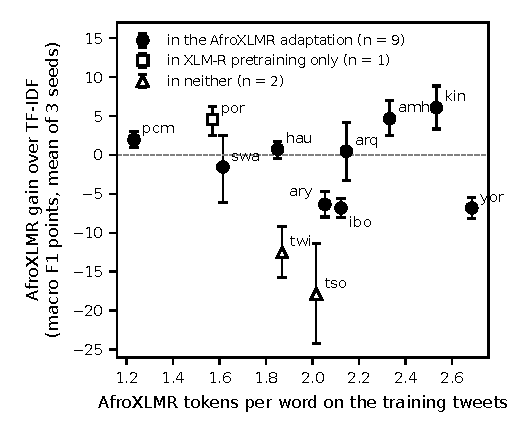
\includegraphics[width=\columnwidth]{fig_gain_vs_tpw.pdf}
\caption{Gain of fine-tuned AfroXLMR over the TF-IDF baseline in macro F1 points (mean of three seeds; error bars: 95 percent paired bootstrap interval over the test tweets, 1,000 resamples) against subword tokens per whitespace word under the AfroXLMR vocabulary on the training tweets, for the twelve AfriSenti languages. Marker shape gives the pretraining coverage. Spearman's $\rho = 0.00$ (95 percent bootstrap interval $-0.72$ to $0.69$, permutation $p = 1.000$, $n = 12$).}
\label{fig:gain}
\end{figure}

\begin{table*}[t]
\centering
\footnotesize
\begin{tabular}{lllrrr}
\toprule
Test & Predictor & Outcome & $\rho$ & 95\% interval & $p$ \\
\midrule
primary & AfroXLMR tokens per word & AfroXLMR $-$ TF-IDF & 0.00 & [-0.72, 0.69] & 1.000 \\
exploratory & LaBSE tokens per word & LaBSE $-$ TF-IDF & 0.13 & [-0.60, 0.71] & 0.675 \\
exploratory & word OOV rate & AfroXLMR $-$ TF-IDF & 0.04 & [-0.55, 0.58] & 0.902 \\
exploratory & word OOV rate & LaBSE $-$ TF-IDF & 0.48 & [-0.16, 0.88] & 0.122 \\
exploratory & training set size (log) & AfroXLMR $-$ TF-IDF & 0.13 & [-0.56, 0.69] & 0.680 \\
exploratory & training set size (log) & LaBSE $-$ TF-IDF & -0.53 & [-0.93, 0.20] & 0.082 \\
exploratory & AfroXLMR tokens per word & AfroXLMR $-$ LaBSE & 0.11 & [-0.47, 0.64] & 0.735 \\
partial, given size & AfroXLMR tokens per word & AfroXLMR $-$ TF-IDF & -0.03 & [-0.77, 0.70] &  \\
partial, given size & LaBSE tokens per word & LaBSE $-$ TF-IDF & 0.25 & [-0.72, 0.79] &  \\
exploratory & AfroXLMR tokens per word & LaBSE tokens per word & 0.88 & [0.57, 0.98] & $<$0.001 \\
\bottomrule
\end{tabular}
\caption{Spearman's $\rho$ across the twelve languages, with 95 percent bootstrap intervals over languages (10,000 resamples) and two-sided permutation $p$-values (10,000 shuffles). The primary test was fixed before the runs; the partial rows remove the rank correlation with the log training size.}
\label{tab:corr}
\end{table*}

\subsection{Retyping and perturbations}
Table~\ref{tab:robust} gives the four robustness conditions as clean minus altered macro F1, so a positive number is a loss. Retyping the Kinyarwanda test set moves the word-level OOV rate from 26.5 to 37.8 percent, the LaBSE tokens per word by 6.2 percent and the AfroXLMR tokens per word by 2.7 percent; the losses are 0.4, 1.2 and 2.3 points, and only the fine-tune's interval excludes zero. The order is the reverse of the token change: the pipeline whose input moved the most at its own level lost the least. My reading is that the character n-grams of the TF-IDF pipeline still match most of a stretched or vowel-dropped word, so the word-level OOV rate overstates what that pipeline sees. Lower-casing costs under one point everywhere. Removing the \texttt{@user} placeholder from the Kinyarwanda test set, which was trained with it in 70 percent of its tweets, costs at most 1.1 points. Adding the placeholder to the Swahili test set, whose training tweets never carry it, costs the two encoders 8.4 and 8.6 points, with 218 changed predictions for LaBSE, while TF-IDF moves by less than half a point with four changed predictions: a token the vectorizer never saw has no feature. The fine-tune's accuracy does not change on that condition (0.617 to 0.619) while its macro F1 falls, so the placeholder pushes it further toward the majority class.

\begin{table*}[t]
\centering
\footnotesize
\begin{tabular}{lrrrr}
\toprule
Condition & Changed & TF-IDF & LaBSE & AfroXLMR \\
\midrule
kin test retyped (texting conventions) & all 1,026 & +0.4 [-1.4, +2.2] & +1.2 [-0.8, +3.1] & +2.3 [+0.9, +4.0] \\
kin test lower-cased & 984 of 1,026 & +0.0 [+0.0, +0.0] & +0.1 [-1.5, +1.8] & +0.7 [-0.5, +1.9] \\
kin test, @user removed & 731 of 1,026 & +1.0 [-0.5, +2.6] & -0.6 [-2.2, +1.0] & +1.1 [+0.1, +2.2] \\
swa test, @user added & 748 of 748 & -0.4 [-0.9, -0.1] & +8.4 [+5.3, +11.6] & +8.6 [+5.3, +11.7] \\
\bottomrule
\end{tabular}
\caption{Clean minus altered macro F1 in points, with 95 percent paired bootstrap intervals, for the retyped Kinyarwanda test set and the three perturbations that copy mismatches found in the released splits.}
\label{tab:robust}
\end{table*}

\subsection{What the released splits contain}
\label{sec:audit}
Near-copies are rare. The share of test tweets with a training tweet at cosine similarity 0.8 or more is below 1 percent in six languages and highest in Yoruba (7.2 percent), Hausa (6.1) and Igbo (4.0); on those near-copies TF-IDF scores 0.93, 0.93 and 0.92 against 0.73, 0.74 and 0.80 on the rest, and the nearest training tweet carries the test label 88 to 96 percent of the time. Removing them would move the Yoruba TF-IDF accuracy by about one point, not by the twelve points it leads LaBSE by, so near-copies do not explain the lexical baseline's strength in the Nigerian languages.

Table~\ref{tab:artifacts} shows what does differ between splits. In Yoruba, Igbo and Hausa, 95 to 99 percent of training tweets contain a capital letter and 0 percent of test tweets do; the AfriSenti paper says in its Section 4.3 that the Nigerian test sets were lower-cased, and the training sets were not. In the same three languages the \texttt{@user} placeholder is in 44, 68 and 99.9 percent of training tweets and in none of the test tweets, and the link placeholder follows the same pattern in Yoruba and Igbo (21 and 25 percent against 0). Amharic and Moroccan Arabic show the reverse: no placeholder in training and \texttt{@user} in 62 and 42 percent of test tweets. Moroccan Arabic also changes script, from 41 percent of training tweets written in Latin letters only to 51 percent in test. Twi and Nigerian Pidgin have no capitals and no placeholders in any split, which suggests they were lower-cased and stripped before release. Both tokenizers are case-sensitive, so the lower-cased test sets reach the models as different token sequences from the training sets. The measured costs of the previous section put these artifacts in perspective: case and a removed placeholder cost about a point, a placeholder that appears only at test time costs the encoders eight.

\begin{table}[t]
\centering
\scriptsize
\setlength{\tabcolsep}{3.5pt}
\begin{tabular}{lrrrrrr}
\toprule
 & \multicolumn{2}{c}{Capital letter} & \multicolumn{2}{c}{@user} & \multicolumn{2}{c}{Link} \\
Lang. & train & test & train & test & train & test \\
\midrule
kin & 96.4 & 95.9 & 70.5 & 71.2 & 32.0 & 29.5 \\
swa & 96.8 & 97.3 & 0.0 & 0.0 & 0.2 & 0.3 \\
tso & 88.4 & 90.2 & 51.5 & 53.9 & 29.4 & 22.8 \\
arq & 4.0 & 4.1 & 93.1 & 93.2 & 0.0 & 0.0 \\
por & 98.3 & 94.6 & 38.5 & 41.3 & 28.7 & 32.4 \\
twi & 0.0 & 0.0 & 0.0 & 0.0 & 0.0 & 0.0 \\
pcm & 0.0 & 0.0 & 0.0 & 0.0 & 0.0 & 0.0 \\
ary & 0.5 & 22.8 & 0.0 & 42.1 & 0.0 & 4.9 \\
amh & 7.5 & 11.7 & 0.0 & 62.3 & 0.0 & 0.0 \\
yor & 98.8 & 0.0 & 43.9 & 0.0 & 21.1 & 0.1 \\
ibo & 96.9 & 0.0 & 68.5 & 0.0 & 25.3 & 0.0 \\
hau & 95.3 & 0.0 & 99.9 & 0.0 & 3.1 & 0.0 \\
\bottomrule
\end{tabular}
\caption{Release artifacts: share of tweets (percent) with a capital letter outside the placeholders, with the \texttt{@user} placeholder, and with the link placeholder, in the training and test splits.}
\label{tab:artifacts}
\end{table}

\subsection{The adversarial suite}
Table~\ref{tab:suite} gives the counts. The ranking of the test sets does not survive the suite. On the 25 new Kinyarwanda items the frozen encoder leads (17 correct) and the fine-tune is second (14.3); on the 24 new Swahili items TF-IDF leads (12) and the fine-tune is last (9.3). Three patterns stand out in the per-item answers. First, the formal register pulls every model toward positive. TF-IDF answered positive on all six formal Kinyarwanda items, two thanks, two neutral notices and two complaints, right twice by the same rule that made it wrong four times; LaBSE did so on five, the fine-tune on four, and the two formal complaints were positive for every one of the five runs, while their casual twins were negative for TF-IDF. Second, TF-IDF reads the Kinyarwanda negation markers as negative: of the twelve negation items it got the four negative ones right, except a rhetorical question, and nothing else; thirteen of its 25 answers on the new Kinyarwanda items are negative. LaBSE read 8 of the 12 negations and the fine-tune 7, both missing the idiom \emph{ntako atagize} (``there is nothing s/he did not do''), which no run read. Third, the Swahili fine-tune answers neutral: 20 of its 24 answers on the new Swahili items, including all eight negative items, and all eight sentences written by the native readers, of which one is neutral. On the 17 reused items the retrained pipelines give the same answer as the models of the preliminary study on every item for TF-IDF and LaBSE and for the seed 42 fine-tune (11 of 17 in both), so the grid reproduces that study to the item.

\begin{table}[t]
\centering
\scriptsize
\setlength{\tabcolsep}{3.5pt}
\begin{tabular}{llrrrr}
\toprule
Items & Category & $n$ & TF-IDF & LaBSE & AfroXLMR \\
\midrule
new, kin & negation & 12 & 3 & 8 & 7 \\
new, kin & mixed & 1 & 0 & 1 & 0 \\
new, kin & register & 12 & 6 & 8 & 7.3 \\
new, kin & all & 25 & 9 & 17 & 14.3 \\
\midrule
new, swa & negation & 16 & 6 & 4 & 4.7 \\
new, swa & register & 8 & 6 & 7 & 4.7 \\
new, swa & all & 24 & 12 & 11 & 9.3 \\
\midrule
reused, kin & negation & 4 & 2 & 2 & 2 \\
reused, kin & sarcasm & 3 & 3 & 0 & 2 \\
reused, kin & mixed & 4 & 2 & 3 & 2.3 \\
reused, kin & code-switching & 3 & 2 & 1 & 2 \\
reused, kin & register & 3 & 1 & 2 & 2 \\
reused, kin & all & 17 & 10 & 8 & 10.3 \\
\bottomrule
\end{tabular}
\caption{Adversarial suite: correct answers of $n$ items per language and category (AfroXLMR: mean over three seeds). New items were written for this paper; reused items come from the preliminary study.}
\label{tab:suite}
\end{table}

\subsection{Compute}
Table~\ref{tab:compute} gives the cost. The twelve TF-IDF runs took 96 s in all and the twelve LaBSE runs 89 s; the 36 fine-tuning runs took 6,578 s, a total inflated by the shared server (one Xitsonga seed took about 700 s where the next seed took 15 s), so it is an upper bound; in the preliminary study the same fine-tune took 38 s per seed on 3,241 Kinyarwanda tweets. Peak GPU memory was 2.25 GiB for LaBSE and 4.92 GiB for the fine-tune. One Kinyarwanda tweet takes 2.0 ms on the CPU with TF-IDF, 8.8 ms on the GPU with LaBSE and 10.9 ms with the fine-tune (131 and 160 ms on the CPU); in one batch, 0.18 ms per tweet on the CPU for TF-IDF and 1.01 and 0.61 ms on the GPU for the two encoders.

\begin{table}[t]
\centering
\scriptsize
\setlength{\tabcolsep}{3.5pt}
\begin{tabular}{lrrrrrrr}
\toprule
 & & Time, & Peak & \multicolumn{2}{c}{GPU ms} & \multicolumn{2}{c}{CPU ms} \\
Pipeline & Runs & all runs & GPU & one & batch & one & batch \\
\midrule
TF-IDF & 12 & 96 s &  &  &  & 2.01 & 0.18 \\
LaBSE & 12 & 89 s & 2.25 GiB & 8.76 & 1.01 & 130.5 &  \\
AfroXLMR & 36 & 6,578 s & 4.92 GiB & 10.86 & 0.61 & 159.5 &  \\
\bottomrule
\end{tabular}
\caption{Compute: runs in the grid, training time over all runs, peak GPU memory, and latency per Kinyarwanda test tweet in milliseconds (200 tweets, five warm-up calls).}
\label{tab:compute}
\end{table}

\section{Discussion}
\textbf{The tax is real, the prediction is not.} Kinyarwanda words take 2.5 subword tokens under the AfroXLMR vocabulary and Nigerian Pidgin words 1.2, and in both the fine-tune beats TF-IDF. Yoruba words take 2.7 and Hausa words 1.9, and in both TF-IDF is as good or better. Across the twelve languages the rank correlation between fertility and the fine-tuning gain is zero, with an interval wide enough to hold a moderate effect of either sign, which is what twelve languages can say. The finding of \citet{lundin2026tokentax}, lower accuracy with higher fertility for frozen large models on a knowledge benchmark, shows no sign of carrying over to a classifier trained on the task's own labeled data, where the encoder's pieces are tuned on the words of the language, however many there are per word.

\textbf{What does separate the languages.} Two things, and they are confounded. The two languages absent from every pretraining list, Xitsonga and Twi, are where fine-tuning loses the most, and the frozen encoder loses there too. Training size works on the two steps in opposite directions: the frozen encoder helps most where training is small, and the fine-tune recovers the most ground where training is large. The third factor is the data itself. The three largest Nigerian sets are where TF-IDF leads by twelve to nineteen points over LaBSE. Near-copies account for about a point of it. The rest fits how those sets were built: NaijaSenti describes collection by emoji and stopword queries with a sentiment-lexicon filter, which puts the labels close to the surface words, and the Nigerian test sets were lower-cased and stripped of their placeholders while their training sets were not, which costs case-sensitive encoders something and a bag of character n-grams almost nothing. A lexical baseline is hard to beat on data collected lexically.

\textbf{Release artifacts are a finding.} The split-level mismatches in Table~\ref{tab:artifacts} are visible to every model and invisible in the published scores, since every system meets the same test set. Their measured costs are small for case and for a removed placeholder and large for a placeholder present only at test time, eight macro F1 points for both encoders on Swahili. Anyone comparing models on AfriSenti compares them on these artifacts too, and the direction of the effect depends on the model family.

\textbf{What the suite says about understanding.} The suite was written after the preliminary study, with the register and negation traps aimed at weaknesses that study had shown, so it is a diagnostic set rather than a benchmark. What it shows is that none of the three pipelines reads the two things it was built to test. A polite formal complaint is positive to all of them: the formal register, with its respectful plurals and official vocabulary, is a positive cue the models learned from training data whose positive class, in Kinyarwanda at least, holds campaign and promotional posts (an observation from the preliminary study). A negation that does not mean ``bad'' is a coin toss for the encoders and a loss for TF-IDF, which learned the Kinyarwanda negation markers as negative features. The Swahili fine-tune's answer to the native-written sentences, neutral on every one, is the quiet failure that out-of-vocabulary input produces in a model that leans on its majority class.

\textbf{Guidance by coverage.} For a language in the AfroXLMR adaptation list with a few thousand labeled tweets, fine-tuning is worth its cost only where the task's own data rewards it, and a frozen encoder with a linear classifier is the safer default: it lost more than ten points to TF-IDF only in the three Nigerian sets, it cost 89 s for twelve languages, and it did not collapse to the majority class. For a language in no pretraining list, TF-IDF with character n-grams was the best of the three in both cases, at 2 ms per tweet on a CPU. In every case the kept models should be scored on items the native speaker wrote for the failure modes that matter, because the test set will not show them.

\section{Conclusion}
Across twelve AfriSenti languages, how many subword tokens a vocabulary spends on a word did not predict how much a fine-tuned encoder gains over a bag of words on that language's sentiment task. Pretraining coverage, training size and the way the data was collected tell more, and the released splits carry artifacts whose cost can be measured and in one case is large. The Kinyarwanda result that started this study was one point in a cloud, and the cloud has a shape, but the shape is not the tokenizer tax. What a native speaker can add is the part no table shows: the items where every model agrees and every model is wrong.

\section*{Limitations}
Twelve languages give the correlation tests little power: the primary interval runs from $-0.72$ to $0.69$, so the result rules out a strong effect, not a moderate one. All twelve come from one dataset, with annotation agreement between 0.41 and 0.66 and about one in five duplicated Kinyarwanda tweets carrying two labels, so part of every score is label noise. Fertility was measured under two vocabularies of the same family and training size, coverage and collection method are confounded with each other and with fertility. Pretraining contamination cannot be ruled out either: both encoders were pretrained on web text that may contain tweets from these sets, and the near-copy audit covers only what the training split shares with the test split. The fine-tune ran three seeds for three epochs with one learning rate, and bfloat16 training is not bit-reproducible, so single seeds move by up to a point across reruns; the means are what is reported. Training times were measured on a shared server and are upper bounds. The adversarial suite holds 66 items, 49 of them new and in two categories only, so its counts are small; the Swahili labels are those of a non-native speaker checked by two native speakers, and the items were written by the same person who knew the models' weaknesses. Zero-shot prompting of an open generative model, closer to the setting of \citet{lundin2026tokentax}, was not run.

\section*{Ethics Statement}
AfriSenti is released under CC BY 4.0, and its tweets were anonymized by the dataset's authors. No tweet on a politically sensitive or violent subject is quoted in this paper.

\section*{Acknowledgments}
Two native speakers of Tanzanian Swahili, who asked to remain anonymous, revised the Swahili items of the suite. This study grew out of a course project at the University of Missouri. I used Claude (Anthropic) for planning, code drafting, debugging and writing assistance; I ran all code myself and checked every claim against the printed output.

\bibliography{references}

\end{document}
